\begin{figure*}[htbp]
  \centering
    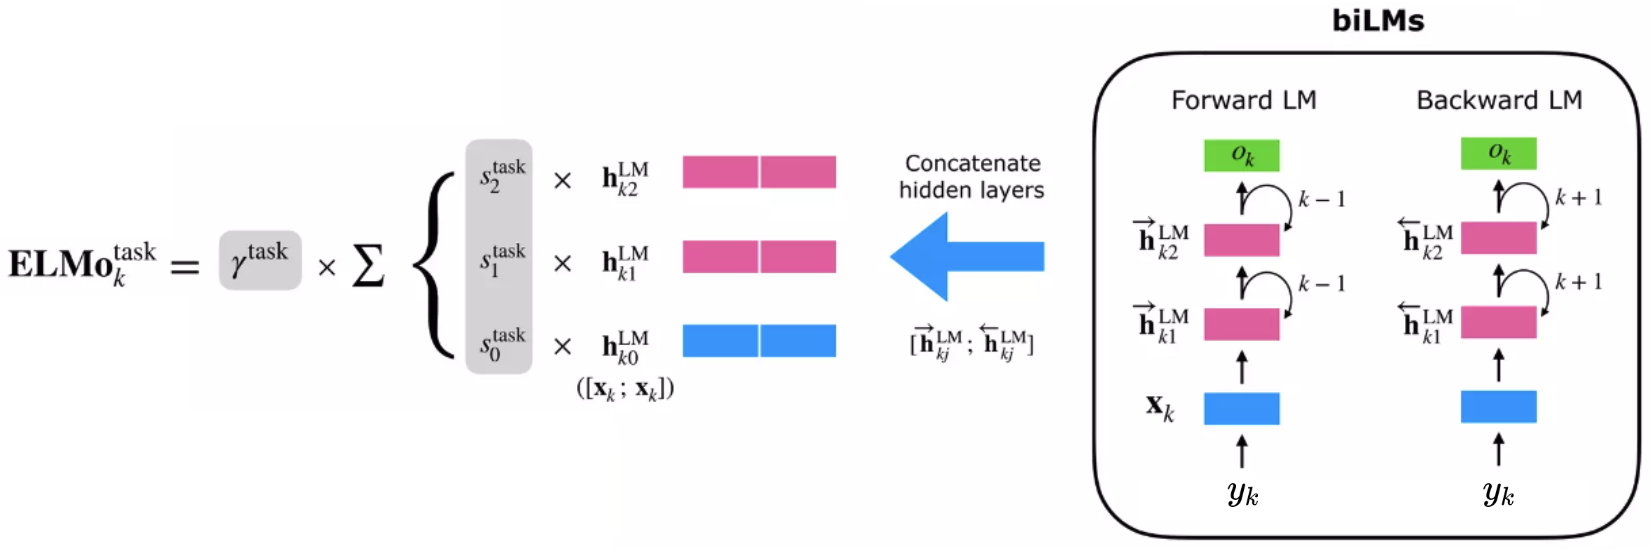
\includegraphics[width=\textwidth]{figures/transfer_learning/ELMo-architecture.png}
  \caption{Illustration of the ELMo model architecture. Hidden representations from forward and backward language models are concatenated in order to yield representations that consider both left and right context. We can then fine-tune weights for these layer-specific representations for various downstream tasks.}
  \label{fig:elmo_architecture}
\end{figure*}


\section{ELMo}

As a first case study of transfer learning based on language models, we consider ELMo \citep{peters-etal-2018-deep}. ELMo was one of the first successful transfer learning models based on language modeling. It leverages the language modeling task to learn word representations, that is, vectors meant to represent the meaning of words. Whereas most previous approaches, such as word2vec \citep{Mikolov2013EfficientEO} and GloVe \citep{pennington2014glove}, trained static word representations, the word representations in ELMo are context-dependent.
The model of \citet{mccann-2017-cove} is another early contextualized word vector model. However, it was pre-trained on machine translation rather than language modeling.
That means that depending on the sentence fed to ELMo, the representation of a particular word will differ in order to reflect the meaning of that particular sentence.


ELMo considers two separate language models, a (standard) forward language model $\pLM(\sym_\tstep \mid \str_{<\tstep})$ as well as a backward language model $\pLMB(\sym_\tstep \mid \str_{>\tstep})\defeq \prod_{\tstep=1}^{\strlen} \pLMB(\sym_\tstep \mid \sym_{\tstep+1}, \dots, \sym_{\strlen})$. Both are implemented by stacking $\layer$ layers of LSTMs, the parameters of which we refer to as $\paramslstmforward$ and $\paramslstmbackward$ respectively. For a given input token $\sym_\tstep$, the forward LSTM layers output context-dependent representations $\hiddenlstmforward{\tstep\layeridx}$, with $\layeridx \in [0,\layer]$ (and analogously, $\hiddenlstmbackward{\tstep\layeridx}$ for the LSTM layers of the backward language model). 
The deepest representations $\hiddenlstmforward{\tstep\layer}$ and $\hiddenlstmbackward{\tstep\layer}$ are fed to a softmax layer to predict the forward and backward probabilities of $\sym_\tstep$. In addition to $\paramslstmforward$ and $\paramslstmbackward$, the parameters for token representations and the softmax layer (denoted together as $\paramselmo$) are tied between the two networks. All parameters are optimized jointly by maximizing the log likelihoods of the forward and backward models: 

\begin{equation}
    \gL_{\texttt{ELMo}}(\params) = \sum_{\idx=1}^{\setsize}\sum_{\tstep=1}^\strlen \log\pLM(\sym_\tstep^{(\idx)}\mid \str_{<\tstep}^{(\idx)}; \paramslstmforward, \paramselmo) + \log\pLMB(\sym_\tstep^{(\idx)}\mid \str_{>\tstep}^{(\idx)}; \paramslstmbackward, \paramselmo)
\end{equation}

Now in order to fine-tune for a specific task, we can use the context-specific representations $\hiddenelmo{\tstep\layeridx}=[\hiddenlstmbackward{\tstep\layeridx};\hiddenlstmforward{\tstep\layeridx}]$. One could simply take the last layer representations $\hiddenelmo{\tstep\layer}$ and use those as input to a separate model that is fine-tuned on another task. The original paper additionally experimented with learning a task-specific representation as a scaled convex combination over the hidden representations, as follows:

\begin{equation}
    \textbf{ELMo}^{\text{task}}_{\tstep} = \vgamma^{\text{task}} \sum_{\layeridx=0}^{\layer} s_\layeridx^{\text{task}} \hiddenelmo{\tstep\layeridx},
\end{equation}
where $\sum_{\layeridx=0}^{\layer} s_\layeridx^{\text{task}}=1$ are the outputs of a softmax function over the hidden representations, and $\vgamma^{\text{task}}\in\mathbb{R}$ is meant to scale the representations.%\mrinmaya{Say these s's are outputs of a softmax. Also the purpose of $\gamma$ is to scale these representations \response{andreas}{Added}} The full pipeline, including the above scheme, is illustrated in \cref{fig:elmo_architecture}.%\mrinmaya{Can we say also how ELMO would be used in practice for a task. See my slides \response{andreas}{Added the paragraph below}}

Now, consider a neural network-based model $\func_{\hat{\params}}$ that is fine-tuned on some downstream task. As input it takes a sequence of representations $(\ervx_1, \dots, \ervx_\strlen)$. These could be some pre-trained static representations or simple one-hot encodings. To improve the model using contextualized information we can concatenate these input representations with the ELMo representations, yielding input on the form $[\ervx_\tstep; \textbf{ELMo}^{\text{task}}_{\tstep}]$. This only changes the input dimension of $\func_{\hat{\params}}$, the rest of the network can remain unchanged, and be further fine-tuned.

\begin{table*}[htbp]
  \centering
    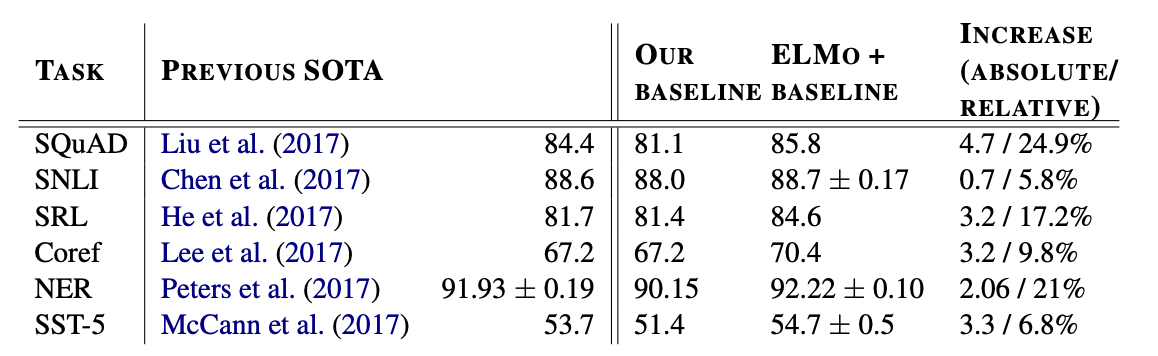
\includegraphics[width=0.9\textwidth]{figures/transfer_learning/elmo-results.png}
  \caption{Results of ELMo on six benchmark tasks, compared to previous state-of-the-art results. The performance metrics vary across the tasks. SNLI and SST-5 are measured by accuracy. SQuAD, SRL and NER are measured by F1. Coref is measuerad by average F1. \TODO{take a PDF-screenshot instead of png}}
  \label{fig:elmo_results}
\end{table*}

ELMo was indeed somewhat of a breakthrough in NLP transfer learning research: By leveraging ELMo representations for other downstream tasks as just described, the original paper was able to beat what was at the time state-of-the-art performance on six different benchmark datasets. These benchmarks included the tasks of question answering, natural language inference, semantic role labeling, coreference resolution, named entity recognition and sentiment analysis. See \Cref{fig:elmo_results} for exact numbers.